$\{Y(t):t \geq 0\}$ is a birth and death process since whenever an indiv


The continuous-time Markov chain is a birth and death process if the following is satisfied
$$P_{i, i+1}(h) = \lambda_i + o(h) \text{ }(\text{as } h\rightarrow 0^+) \text{ for } i \geq 0$$
$$P_{i, i-1}(h) = \mu_i + o(h) \text{ }(\text{as } h\rightarrow 0^+) \text{ for } i \geq 1$$
$$P_{i, i+1}(h) = 1 - (\lambda_i + \mu_i)h+ o(h) \text{ }(\text{as } h\rightarrow 0^+) \text{ for } i \geq 0$$
$$ P_{ij} = \delta_{ij} = 0 \text{ for } i \neq j $$
$$ P_{ij} = \delta_{ij} = 1 \text{ for } i = j $$
$$\mu_0 = 0, \lambda_0 > 0\text{ and } \mu_i, \lambda_i > 0 \text{ for } i\geq1.$$

Alternative DEF:
Whenever you jump to state i, two competing processes start: 
$$\text{1) } T_1  = \text{ "time until birth" } \sim \text{ Exp}(\lambda_i)$$
$$\text{2) } T_2 = \text{ "time until death" } \sim \text{ Exp}(\mu_i)$$

The transition diagram for $\{Y(t): t\geq 0\}$ is illustrated in figure \ref{transdiagramY}.

\begin{figure}
    \centering
    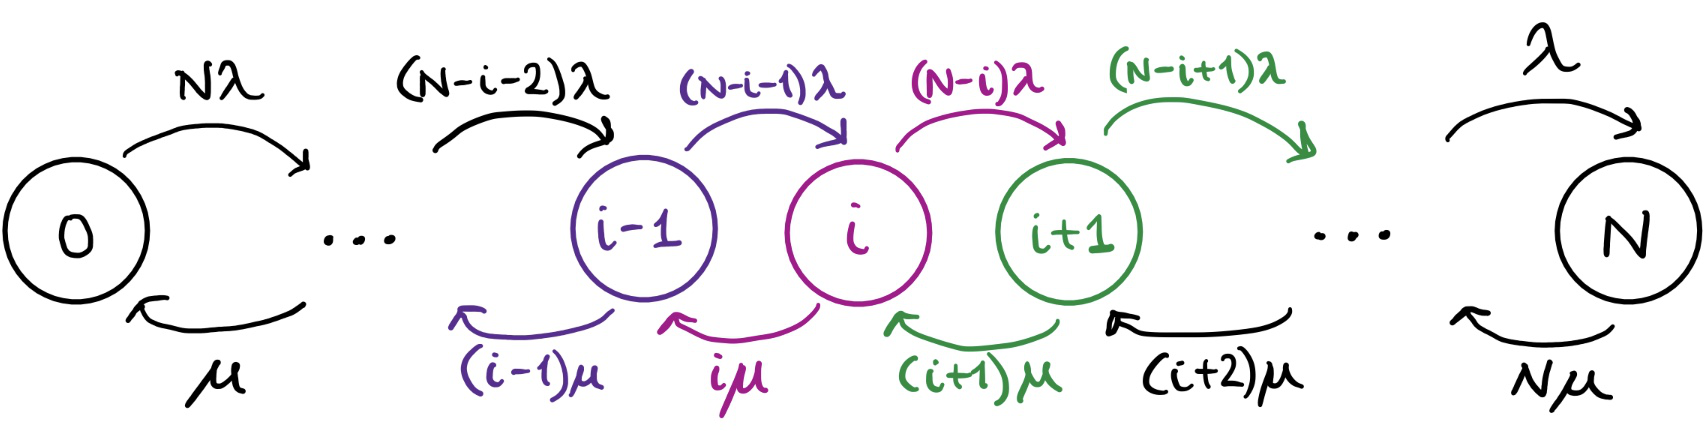
\includegraphics[width=140mm]{TransDiag1F.png}
    \caption{Transition diagram of $\{Y(t):t \geq 0 \}$. $N$ is defined as the number of individual in a population, in this case $5.26 \text{ millions.}$}
    \label{transdiagramY}
\end{figure}